\section{Standard Model}
\label{sec:SM}
%All known fundamental particles and forces can be describe by the standard model (SM). Only gravity is not included in the SM.
%One of the greatest success is that the SM was capable of predicting particles like the top quark before they were discovered.
%Since its development many experiments have performed precision measurements and up to now no deviation has been found.
%However there are some unresolved problems.
%This section describes the fundamental forces along with all particles and explains briefly the Higgs mechanism which is needed for particles to gather mass and generate the electroweak symmetry breaking.


During the 20th century the Standard Model of particle physics (SM) has been developed.  
The SM is a quantum field theory based on gauge invariance including all fundamental particles, leptons and quarks, and three fundamental forces, Quantum Chromodynamics (QCD)(Sec.~\ref{sec:qcd}) and Quantum Electrodynamics (QED)(Sec.~\ref{sec:qed}) unified with the weak force to the electro-weak force (Sec.~\ref{sec:electro-weak}). In addition the Higgs mechanism (Sec.~\ref{sec:higgs}) is introduced in order to generate masses for the weak gauge bosons and all fermions.% The interactions are introduced via three gauge symmetry groups (Sec. \ref{sec:gauge}).\\
Except for the Higgs-boson all particles and forces have been found experimentally. However, new LHC and Tevatron results have found consistently candidate events for a Higgs-boson with a mass of about 126 GeV\cite{ATLAS-CONF-2012-019}\cite{CMS-PAS-HIG-12-008}\cite{bib:TevatronHiggs:2011cb}. \\
This section covers a short introduction to gauge theory and the Dirac equation followed by the derivation of Quantum Electrodynamics (QED) from gauge theory and a phenomenological description of the strong force (QCD), the weak force and its unification with QED. Also the concept of the Higgs mechanism is briefly described. The last part covers some of the unresolved problems within the SM suggesting a more fundamental theory. 

%The SM can only be seen as a low energy approximation of a more fundamental theory
%re strong reasons why the SM can not be seen as a complete theory but only a low energy approximation of a more fundamental theory.\\ 


%Particles physics focuses on the investigation and explanation of the smallest constituents of matter and how they interact. The aim is to understand how the world around us is formed and what keeps it together on smallest scales.\\
%During the 20th century the so called Standard Model of Particle Physics (SM), has been developed. The SM consists of the basic ingredients of matter, leptons and quarks (see sec.\ref{subsec:fundamental_particles}) and the fundamental forces, the quantum chromodynamics (sec. \ref{sec:qcd}) the electro-weak force (sec.\ref{sec:qed},\ref{sec:electro-weak}) and the Higgs mechanism(sec.\ref{sec:higgs}). The name Model has been chosen because their are strong reasons why the SM is can not be seen as a complete theory but only a low energy approximation of a more fundamental theory.\\ 
%To honor one of the main principles of physics, make the least assumptions and input for describe and predict as much as possible, the SM has been build on very few ingredients. The fundamental particles and interactions via forces are based on very fundamental symmetry principles (see sec.\ref{sec:gauge}).\\
%One of the greatest achievements and success of the SM is the discovery of the $W$ and $Z$ Vector-Boson which had been predicted also the validation of the SM over many magnitudes of energy from a few eV up to the TeV regime by experiments like LEP\cite{bib:Barate:2003sz}\cite{bib:LEPEWKWG:ZPolse2005}, TEVATRON\cite{LEPEWKWG:2010vi}\cite{bib:Abe:1995hr}\cite{bib:Abachi:1995iq}, and HERA has to be honored.\\
%One crucial ingredient to the SM is the Higgs Mechanism which is introduces for electroweak symmetry breaking in order to make the $Z$ and $W$ boson massive and is also an elegant way for all other particles to gather masses.\\
%All particles predicted by the SM have been discovered but the Higgs Boson which is a consequence of the Higgs Mechanism. However new results from the two LHC experiments ATLAS and CMS and TEVATRON consistently yield hints to a Higgs Boson with a mass of about 126~GeV.\\
%Despite these successes the SM suffers from some short comes (sec. \ref{sec:SM_problems}).\\
%This section introduces the relevant theoretical structures of the SM (sec.\ref{sec:gauge}), particles (sec.\ref{subsec:fundamental_particles}) and forces (sec.\ref{subsec:fundamental_forces}).\\
%For the whole thesis natural units are used setting $\hbar = c = G = k_{B} = 1$ (with $\hbar$ being the reduced Planck constant, $c$ the speed of light, $G$ gravitational constant and $k_{B}$ being the Boltzmann constant).
%One main principle of physics is to explain nature with the least possible assumptions and derive and predict as much as possible from the least input. Under this premise the Standard Model (SM) of particle physics has been developed. \\
%The SM is a theory able to describe all fundamental particles and forces from a few very basic assumption. It has been developed to combine special relativity with quantum mechanics by gauge theories. From very simple symmetry demands particle interactions can be introduced and the forces are predicted.\\ 
%However the SM is not able to explain the size of the masses of the particles or why the positive charge of the proton is to a very high precision of the same strength as the negative charge of the electron.  parameters have to be measured and enter the model without any justification of size.  Also all efforts to merge the SM with general relativity have failed.\\
%Another main problem arises from astro physical indirect observations of non SM matter called dark matter. SM particles only make up 4.6\% of the total energy in the universe. About 72\% are maid up by an even more exotic energy the so called dark energy. The dark matter is expected to make up more than 23\% of the total energy in the universe. Thus extensions of the SM are obviously needed to become a full valid theory. One very famous Ansatz is supersymmetrie which is discussed in sec.\ref{sec:susy}.\\ 
%Despite these short comes, the SM has been incredible successful in describing experimental data and predicting particles before they were discovered. All experiments, mainly collider experiments, have shown no significant deviation from the SM expectation. However one has to mention that all particles included in the SM have been found but the Higgs boson which is crucial for the Higgs mechanism which is needed for particles to obtain masses. But indirect indications support this mechanism quite strongly.\\
%This section describes the fundamental particles, the three fundamental forces and the higgs mechanism in the following subsections.


\subsection{The Dirac equation and gauge groups}
\label{sec:gauge}
This section discusses the Dirac equation followed by an overview of the gauge groups, which introduce the three fundamental interactions.\\

By combining quantum mechanics and special relativity the relativistic energy momentum relationship ($m^{2}=E^{2}-p^{2}$) had to be modified in analogy to the Schroedinger equation by replacing the energy $E$ and the momentum $p$ by the quantum mechanical operators $\hat p = -i\nabla$ and $\hat E = i \frac{\partial}{\partial t}$.\\
The resulting Dirac equation describes all fundamental fermions with spin $1/2$ by four component spinor fields $\Psi$($\bar{\Psi}$)\footnote{The adjoint spinor $\bar{\Psi}=\Psi^\dagger \gamma^0$ with $\Psi^\dagger$ being the conjugated transpose of $\Psi$ and $\gamma^0$ one gamma matrices\cite{bib:Schmuser:FeynmanGraphs}.}:
$$ \mathcal{L}_{Dirac} = \bar{\Psi}i\gamma^{\mu}\partial_{\mu}\Psi-m \bar{\Psi}\Psi  .$$\
These four components introduce two solutions with negative energy. These solutions can be interpreted as particles moving back in time called anti-particles. These anti-particles carry the same but opposite charge.\\
Fig.~\ref{fig:particles} shows all fermions and gauge bosons included in the SM.
The fundamental fermions can be divided into two species, leptons and quarks.\\
The charges of a particle determine via which force it interacts. All fermions except neutrinos are weakly and electrically charged. Quarks inherit also a color charge. Neutrinos only interact weakly thus carrying only a weak charge. 
\begin{figure}[tbhn]
\begin{center}
\begin{tabular}{c}
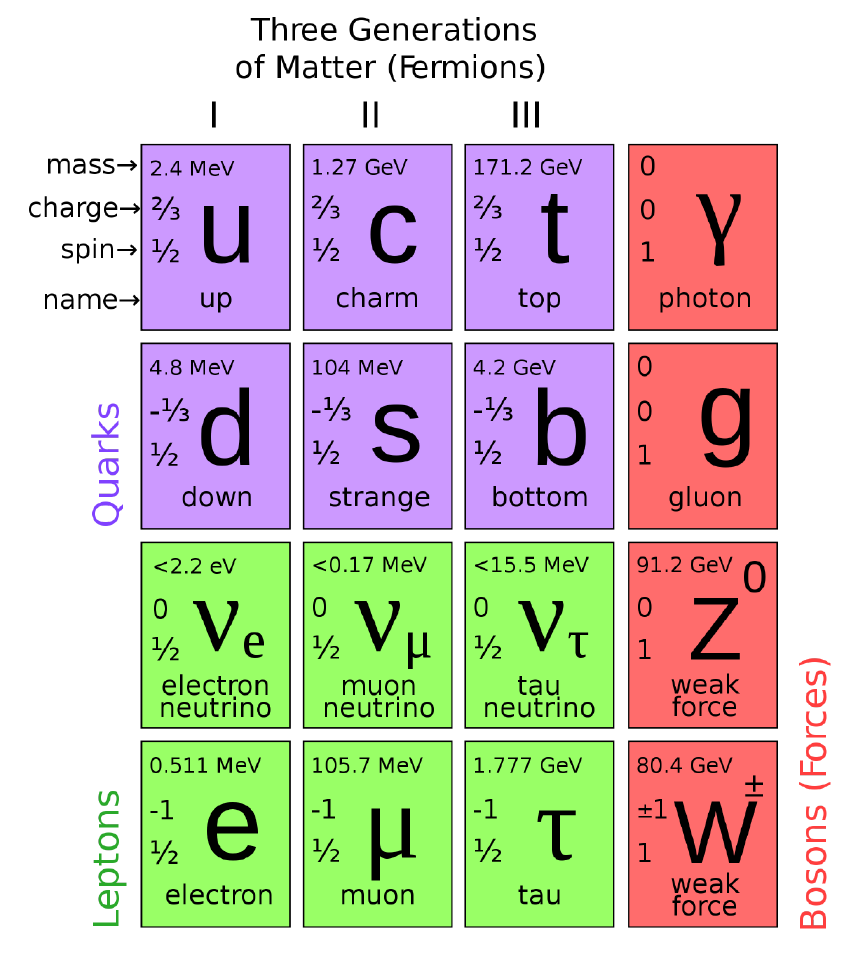
\includegraphics[width=0.65\textwidth]{theory/particles.png}


\end{tabular}
\end{center}
\caption{This figure contains fermions and gauge bosons of the SM. The Higgs boson is not included since its existents has still not been verified by experiments.}
\label{fig:particles}
\end{figure}


%\begin{table}[htb]
%\begin{center}
 %   \begin{tabular}{l|lll}
%        
%        leptons         & $\nu_{e}$ & $\nu_{\mu}$ & $\nu_{\tau}$ \\
%		        & $e$ & $\mu$ & $\tau$ \\ \hline
%        quarks   	& $u$ & $c$ & $t$ \\
%                        & $d$ & $s$ & $b$ \\
%        
%
%    \end{tabular}
%\caption{The fundamental particles of the Standard Model.}
%\end{center}
%\label{tab:particles}
%\end{table}
The three forces are introduced by gauge symmetry groups ($SU(n)$):
\begin{enumerate}
 \item $U(1)_{Y}$: Phase rotation introducing the electromagnetic forces (Sec.~\ref{sec:qed}).
 \item $SU(2)_{L}$: Weak isospin rotation explaining the weak force, combined with the $U(1)_{Y}$ to the electroweak force (Sec.~\ref{sec:electro-weak}).
 \item $SU(3)_{C}$: Rotation of the color charge leading to the strong force (Sec.~\ref{sec:qcd}).
\end{enumerate}
To keep this thesis concise while including all necessary theoretical explanations gauge invariance is only discussed in detail for QED. The weak, electro-weak unification and the strong force is only described phenomenologically.
\subsection{Quantum Electrodynamics (QED)}
\label{sec:qed}
%At the beginning of the 20th century quantum mechanics (QM) and special relativity were introduced. Attempts of combining these two theories for particles resulted in two equations for free particles. The first fundamental equation is the %Klein-Gorden-Equation describing free spin 0 particles.\\
%The second equation was formulated by Dirac and describing spin 1/2 particles. Both equations predict particles with a negative mass which lead at first to abandoning these equations. Later they were rehabilitated by interpreting these solutions as anti particles which move back in time. These particles were also discovered later.
This section demonstrates how invariance under a $U(n)$ symmetry group leads to the introduction of forces. This is being discussed for $U(1)$ with the electric charge $q$ as generator leading to electromagnetic interactions.\\ 
The basic idea of invariance is described by the Noether Theorem\cite{bib:Schmuser:FeynmanGraphs} stating that invariance under a global $U(1)$ phase transition $\Psi\rightarrow \Psi e^{-i\alpha}$ leads to the conservation of a charge $q$ and the corresponding current $J^{\mu} = q\bar{\Psi} \gamma^{\mu}\Psi$. 
The Dirac equation is invariant under such a global phase transition:
$$ \mathcal{L}_{Dirac}(\Psi \rightarrow \Psi e^{-i\alpha},\bar{\Psi} \rightarrow \bar{\Psi} e^{+i\alpha} ) =  \mathcal{L}_{Dirac}(\Psi ,\bar{\Psi} ) $$\\
This also implies that the current and thus the electric charge is conserved.\\
The interaction of particles via the electromagnetic force can be introduced by requiring invariance of the Lagrangian under local gauge transformations $U(1)$ depending on the space-time $x$:
$$ \Psi \rightarrow \Psi e^{-i\alpha(x)}.$$ 
With the usual space time derivatives $\partial_{\mu}$ this is not possible. To restore local invariance the space time derivative has to be modified by including a new gauge field $A_{\mu}$ with the following transformation:
$$ A'_{\mu} = A_{\mu}-\frac{1}{e}\partial_{\mu} \alpha(x).$$
The partial derivate is substituted by the covariant derivative $D_{\mu}$ defined as
$$ D_{\mu}= \partial_{\mu}-ieA_{\mu}   $$
resulting in the local gauge invariant Lagrangian: 
$$  \mathcal{L} =  \bar{\Psi}i\gamma^{\mu}\partial_{\mu}\Psi-m \bar{\Psi}\Psi +e \bar{\Psi}i\gamma^{\mu}\Psi A_{\mu}$$
The additional term describes the interaction of the photon $A_{\mu}$ with the fermion. An additional term $F_{\mu\nu} = \partial_{\mu}A_{\nu}-\partial_{\nu}A_{\mu}$\footnote{This is the antisymmetric field strength tensor known from classical electrodynamics.} has to be added to include the energy stored in the electromagnetic field:
$$  \mathcal{L} =  \bar{\Psi}i\gamma^{\mu}\partial_{\mu}\Psi-m \bar{\Psi}\Psi +e \bar{\Psi}i\gamma^{\mu}\Psi A_{\mu} - \frac{1}{4}F^{\mu\nu}F_{\mu\nu}.$$
This is the full QED Lagrangian including the kinetic energy of the particle and its mass together with the interaction of the particle with the Photon and the energy stored in the electromagnetic field. Similar calculations for $SU(2)_L$ and $SU(3)_{C}$ lead to weak and strong interactions. 


\subsection{The weak force and the electroweak unification}
\label{sec:electro-weak}
The weak force can be introduced by the $SU(2)_L$ group with the three Pauli matrices as generators. The $Z$ and the \W bosons are introduced as gauge bosons. In contrast to the other gauge bosons the $Z$ and \W bosons have a mass of $M_{W}=80.4$ GeV and $M_{Z}=91.2$ GeV. The resulting mass terms are not gauge invariant. Instead of direct mass terms the $Z$ and \W couple to the Higgs field (Sec.~\ref{sec:higgs}), which introduces gauge invariant indirect mass terms.\\
The weak force has been found to be maximally parity\footnote{Parity being invariance of physics under space inversion eg. $\vec x\rightarrow -x$} violating leading to exclusive left-handed\footnote{The projection of the spin vector on the momentum vector has a positive sign.} weak interactions for particles and right handed interactions for anti-particles.
The masses of the vector bosons suppresses interactions above the natural range of $10^{-18}$m, determined by the Heisenberg uncertainty principle, making the weak force appear to be weak at energies below ~100 GeV. \\
%The interaction can be written as:
%  \begin{equation}
% J^{\mu}_{weak} = \frac{1}{2}\bar{\Psi}_{1}(V^{\mu}-A^{\mu}\Psi_{2}).
%\end{equation}
%The important point is the V-A componentn in the brackets leading to maximum parity violation.
%The weak force had been introduced to explain the experimental observed $\beta$-decay. he weak force is violating parity (parity being invariance of physics under space inversion eg. $x\rightarrow -x$) making it couple only to left-handed particles. In analogy to the electromagnetic force a field quant had been introduced the $W^{+}\&W^{-}\&Z$ boson. In contrast the weak force is maximal parity violation. This leads to the structure of vector-axialvektor (V-A). The resulting weak current is being described by:
The electroweak unification describes the weak and the electromagnetic force as two aspects of the same force.
The combination can be achieved with a $SU(2)_L \times U(1)_{Y}$ group. The obtained covariant derivative $D^{\mu}$ includes 4 generators $B^{\mu}$ and $W_i^\mu$ with $i=1,2,3$.  
\begin{equation}
 D^{\mu} =  \partial^{\mu} + \frac{i}{2}g\vec \tau_i \cdot \vec W^{\mu}_i + i \frac{g^\prime}{2}YB^{\mu}
\end{equation}
with $g,g^\prime$ being coupling constants, $\tau_{i}$ defined to be the Pauli matrices.
The \W are now mixtures of the $W_{1,2}$ fields:
$$ W^{\pm} = \frac{W_1\pm i W_2}{\sqrt{2}} .$$
The $A^{\nu}$ and $Z^\nu$ are orthogonal linear combinations of the $W_3$ and $B$ fields related via the Weinberg angel $\vartheta_W = 28^\circ$ which had to measured by experiments\cite{bib:LEPEWKWG:ZPolse2005}.
$$ A^\mu =  B^\mu\text{cos}\vartheta_W +  W_{3}^\mu\text{sin}\vartheta_W $$ 
$$ Z^\mu = - B^\mu\text{sin}\vartheta_W +  W_{3}^\mu\text{cos}\vartheta_W $$
The fields $W_{1,2}$ mix to form the charged current. The electromagnetic force now couples via the hypercharge $Y$ (instead of the plain electric charge (q)):
To account for the exclusive coupling of the weak force to left handed particles $\vec T=\frac{1}{2}\vec \tau$ is defined for left handed and $\vec T = 0$ for right handed particles. The electromagnetic force still couples to both handed particles because $Y\ne 0$.\\

 
\subsection{QCD}
\label{sec:qcd}
The third force which is included in the SM is the strong force with the associated color charge and gluons as gauge bosons. The only particles carrying color charges are quarks\footnote{Anti quarks carry an anti-color.} and gluons. Experiments have shown that the color charge comes in three options introducing a new degree of freedom\footnote{For example the ratio of $e_{+}e_{-}\rightarrow \frac{hadrons}{\mu_{+}\mu_{-}}$ being three times larger than expected suggesting a new degree of freedom.}.\\ 
The gauge structure of this force is the $SU(3)_{C}$ group which is similar to the $U(1)$ group. The more complex structure of the $SU(3)_C$ leads to eight color charged gauge bosons\footnote{Either one color or anti color.} and to three and four vertex gluon-gluon interactions. The charged gauge bosons lead to the consequence that the strong force increases over distance resulting in the exclusive existence of color neutral bound states of quarks\footnote{A bound state is considered color neutral when it either consists of one color and its anti color or includes all three colors.} called hadrons. Two different kind of hadrons have been observed. Baryons, consisting of three quarks, each carrying a different color and mesons which consist of a quark and an anti-quark carrying the same color and anti-color respectively.\\
For example the proton consists of quarks and gluons called partons which have to be measured by experiments like HERA\cite{bib:CombinedHERA:2009wt}.\\
The residual of the strong force is responsible for keeping the nucleons together.



\subsection{The Higgs Mechanism}
\label{sec:higgs}
The symmetry of the $SU_{Y}(1) \times SU_{L}(2)$ has to be broken to give masses to the weak vector bosons while preserving gauge invariance. Also the photon and the gluons have to remain massless.\\
Peter Higgs\cite{PhysRevLett.13.508} among others introduced a rather simple solution to this problem. \\
His idea was to introduce a new underlaying field called Higgs field which is present everywhere in space with a degenerated\footnote{i.e. no longer invariant under symmetry transformation} lowest energy state (vacuum expectation value). The corresponding Lagrangian remains gauge invariant. The \W and $Z$ gauge boson can now couple to this field resulting in mass gathering proportional to the strength of the coupling. This symmetry breaking can be achieved while leaving the $U(1)_Y \times SU(2)_L$ symmetry unbroken therefore gauge invariant and leaving the photon massless. The $SU(3)_C$ is also not influenced.\\ 
The simplest way to produce such a so called ''spontaneous'' symmetry breaking is a complex scalar $SU(2)$ doublet with a non zero vacuum expectation value:
\begin{equation}
 \Phi(x) = \binom{\Phi_a(x)}{\Phi_b(x)}
\end{equation}
This potential can also be expressed in its four independent fields $\eta_i$ and a constant $v$:
\begin{equation}
 \Phi(x) = \frac{1}{\sqrt{2}} \binom{\eta_1(x)+i\eta_2(x)}{v+\eta_3(x)+i\eta_4(x)}
\end{equation}
With a gauge transformation $\eta_{1,2,4}$ can be absorbed by the boson fields \W and $Z$ resulting in indirect mass terms. The remaining potential
\begin{equation}
\label{eq:higgsPotential}
 \Phi(x) = \frac{1}{\sqrt{2}} \binom{0}{v+\eta_3(x)}
\end{equation}
is now independent of $\eta_{1,2,4}$.
The corresponding gauge invariant Lagrangian is:
\begin{equation}
 \mathcal{L}_\Phi(x) = (D^\mu\phi(x))(D_\mu\phi(x))-\mu^2|\phi(x)|^2-\lambda|\phi(x)|^4-\frac{1}{4}F^{\mu\nu}(x)F_{\mu\nu}(x)
\end{equation}
with $\phi(x)$ being the scalar Higgs field, $F^{\mu\nu}(x)$ the Lagrangian density of the free field, $D^\mu$ the covariant derivative, $\mu^2$ and $\lambda$ being real parameters. No mass-term for the $\gamma$ is being introduced therefore the $\gamma$ remains massless. A minimum of the potential exists at
$$\nu = \sqrt{\frac{-\mu^2}{\lambda}} $$ 
when $-\mu^2 > 0$ and if $\lambda$ is a real parameter. This minimum can be identified with the vacuum expectation value of the Higgs field, also included in Eq.~\ref{eq:higgsPotential}. A massive spin 0 Higgs boson with the mass of $M_H = \sqrt{-2\mu^2}$ is the consequence of the remaining free Higgs field $\eta_3(x)$.\\
In addition to the mass generation of the weak vector bosons the Higgs mechanism provides also an elegant way for fermions to acquire masses\footnote{In principle neutrinos could also gather masses in the same way but the SM assumes them to be massless.}.
%The potential is rotation symmetric around the origin and has a minimum $v$ at $ v = \frac{\mu}{\lambda}$ as can be seen in fig.\ref{fig:higgs}. Since at $v=0$ no minimum exists and nature always realizes the condition of lowest energy the by construction rotation symmetry is broken and the vacuum expectation value of the Higgs Field is $\frac{v}{\sqrt{2}}\ne 0$.\\ 
%Terms introduced when making the Lagrangian gauge invariance lead to self coupling of the Higgs potential resulting in a massive vector boson the Higgs boson with a bare mass of $ M_{H}=\sqrt{-2\mu^{2}} $. Since $\mu$ is a free parameter the mass of the Higgs boson can not be calculated however precision measurements at LEP exclude a Higgs Boson with masses less than $114$~GeV and masses of more than $600$~GeV are also disfavored. CMS, Atlas and the Tevatron have discovered coherent excesses around $124$~GeV, but the statistical significance is not yet enough for a discovery.\\ 
%The Lagrangian of charged (electric and/or color) fermions can also not contain mass terms while being gauge invariant. However the Higgs mechanism provides also the possibility for fermions to gather masses. The mass term $m_{a}=\lambda_{a}\frac{v}{\sqrt{2}}$ with $a$ being any charged lepton or quark describes the coupling of the fermions to the Higgs field and leads to mass gathering. The coupling constant is a free parameter making the Higgs mechanism able to give to all particles masses but does not explain why the masses are from such different magnitudes.\\
%Neutrinos could in principle gather with the same mechanism masses but are not included in the standard definition.



\section{Open questions and problems of the SM}
\label{sec:SM_problems}
Despite all achievements of the SM in not only describing but predicting particles and interactions it can only be seen as a low energy approximation of a more fundamental theory. The following list provides some short comings of the SM and experimental results hinting towards new physics for which a popular approach will be discussed in the following chapter. 

\begin{itemize}
 \item The weak and electromagnetic force have been unified suggesting the idea of unifying every force within a theory of everything. Such Grand Unified Theories (GUTs), unify the electro-weak and the strong force at an energy around $10^{15}$~GeV in a gauge group $G$ with one single coupling. The SM can not provide such a unification at such a scale. 

 \item All the particles masses can not be predicted within the SM but have to be measured. Further the exact same value of the electric charge for the electron and the proton can not be explained. Also at very high energies radiative corrections to certain processes diverge leading to unitarity violation.

 \item Astrophysical observations have shown discrepancies between expected mass distributions calculated from galaxy gravitational lensing and the visible amount of matter, suggesting a huge amount of dark matter, about 23\% of all energy within the universe \cite{Bertone2005279}. Dark matter does not interact electromagnetically or strongly making it invisible to direct observations. The neutrinos are the only candidates within the SM for such matter but observations require dark matter to be a lot heavier than the upper limit on the neutrino masses. 

 \item Another problem within the SM is the so called ''Naturalness''. The bare Higgs mass $M_{H}$ introduced in Sec.~\ref{sec:higgs} has to be corrected by higher order quadratic loop corrections. If the SM is valid up to the Plank scale ($10^{19}$~GeV), at which gravity becomes as strong as the other forces, loop corrections would increase the Higgs mass significantly. To reduce the mass of the Higgs boson to the favored O(100 GeV) regime, so called ''fine tuning'' is needed. Different independent loop corrections with opposite sign would have to cancel each other to a precision of $10^{-31}$ which is not convincing.

 \item A different approach to solve the Naturalness problem is the introduction of a cut-off energy scale at which new physics is expected. A cut-off at the TeV scale solves the Naturalness problem by demanding new particles with such a mass. Supersymmetry as discussed in Sec.~\ref{sec:susy} can provides such particles and therefore is believed to be realized at the TeV scale making it potentially discoverable by LHC experiments.

 \item Furthermore every attempt to combine gravity and the SM has failed so far.

 \item Also the observed asymmetry of matter and anti-matter can not be explained.

\end{itemize}
%In order to bring the mass of the Higgs Boson to the GeV scale which is in favor of many experimental and theoretical results finine tuning is need which would mean a precision of $10^{34}$ in the Lagrangian mass parameter.\\
These reasons among others lead to the assumption that the SM can only be seen as a low energy approximation of a more fundamental theory.\\




%Several cosomological observations suggest the existing of an additional form of matter called dark matter. Dark matter interacts only weakly and via gravity making it invisible to electromagnetic observations. From measurments of rotation curves the dominating force gravity does not explain how stars are moving unless additional matter is present. Neutrinos interact only weakly and if they are not massless via grvaity but from calculations of the early univers dark matter has to be ``cold'', meaning that the particles have to be non relativistic and a lot heavier than the upper limits on the neutrino masses.\\

%Another problem within the SM is the so called  ``Naturalness of the SM''. The plain Higgs mass $M_{H}$ introduced in sec.\ref{sec:higgs} has to be corrected by higher order loop corrections. If the SM is valid to very high energies up to the Plank scale ($10^{19}$~GeV) at which gravity becomes compatibly strong to the other forces loop corrections would increase the Higgs mass significantly. To reduce the mass of the higgs boson to the favoured GeV regime so called ``fine tuning`` is needed. Different independent loop corrections with opposite sign would have to cancel each other to a precision of $10^{-31}$ which is not convincing.\\

%One of the most obvious short comes of the SM is the lack of integrating gravity. Also the observed asymmetry of matter and anti-matter can not be explained.

\section{Supersymmetry}
\label{sec:susy}
Many theories are available which solve some of theses short comings. A very elegant approach of solving the fine tuning problem and providing a dark matter candidate is Supersymmetry (SUSY). Since this thesis focuses on the search for new physics and especially for SUSY particles an introduction to SUSY will be presented in the next section.
Supersymmetry (SUSY) is the last possible symmetry operation which can be incorporated into the Poincar$\acute e$ group\cite{bib:Aitchison:Susy}. The SUSY generator $Q$ relates fermions and bosons and in its simplest version introduces for each SM particle a supersymmetric partner with a shift in spin of 1/2. Therefore, the SUSY partners of the fermions are bosons with spin 0 called sfermions and the partners of the SM gauge bosons are spin 1/2 fermions called gauginos. In addition another Higgs doublet has to be introduced resulting in five Higgs bosons instead of the one predicted by the SM. The color neutral gauginos and the higgsinos mix to form four charged charginos $\chi^{\pm}_{1,2}$ and four neutral neutralinos $\chi^{0}_{1-4}$.\\
The generator $Q$ commutes with all SM generators resulting in identical quantum numbers and masses of the related particles.\\
Besides the argument that it can in principle be added to the Poincar$\acute e$ group SUSY can also solves many problems of the SM for example the ''Naturalness'' problem. The quadratic loop corrections from SM particles are countered by the SUSY particles that enter with opposite sign.\\
SUSY allows terms which violate baryon- and lepton-number conservation. One consequence is that the proton becomes unstable. The decay is mediated by the product of one lepton- and one baryon-number violating term. The lower limit on the life time of the proton has been found to be $6.6 \cdot 10^{33}$ years \cite{Ahmed:2003sy}\cite{PhysRevLett.102.141801} putting tight boundaries on the decay and therefore on the corresponding terms in the Lagrangian.\\
To recover the proton stability a new conserved quantity, $R$-party, is introduced:
$$ R = (-1)^{3(B-L)+2S}$$
with $B$ being the baryon-number, $L$ the lepton-number and $S$ the spin. SM particles have $R=1$ and SUSY particles have $R=-1$ prohibiting the mixing between SM and SUSY particles.\\
An interesting consequence of R-parity conservation is the stability of the lightest supersymmetric particle (LSP) making it a natural candidate for Dark Matter if it interacts only weakly.\\
So far extensive searches have been conducted for SUSY but none has found any direct evidence for its existents yet (eg.\cite{D0Limits}\cite{CDFLimits}\cite{L3SUSY}). The SUSY particles have to have the same mass as the SM partners but no such particles have been found. This problem can be solved when SUSY is a broken symmetry. For soft broken SUSY more than 100 new free parameters have to be introduced in the most general case.\\
The breaking mechanism is believed to take place at the GUT scale in a so called ''hidden sector'' which is decoupled from the observable universe below the breaking scale. The mass term breaking is mediated via messenger interaction mediated to the observable universe. All soft breaking mechanisms involve gravity as messenger interaction. For mSUGRA gravity is assumed to be the only one.
%Among others gauge-meditated breaking where additional gauge interactions are assumed to communicate the effects of SUSY breaking from the hidden to the observable sector and gravity-mediated breaking where gravitational interactions transmit the breaking have been developed.



\subsection{SUSY breaking in the Model of Minimal Supergravity and the cMSSM}
\label{sec:msugra}
Minimal Supergravity Models (mSUGRA) are favored for presenting experimental results since they include only five free parameters which makes result interpretation easier.\\
In mSUGRA the mass breaking from the hidden sector is transmitted via gravity\footnote{ The graviton couples to the energy-momentum tensor for matter from general relativity. Still the Supergravity Lagrangian has some non-renormalizable parts. Therefore this can not be seen as a proper implementation of gravity but at best as a low-energy approximation.}.
The large amount of over 100 free parameters is reduced to only five by implying that the strength of all gauge coupling parameters become equally strong and unification of the common scalar and gaugino mass breaking terms at the GUT scale\footnote{$\Lambda \approx 10^{16}$ GeV}. The remaining free parameters are:
\begin{equation}
 m_0,m_{1/2},A_0,\text{tan}\beta,\text{sign}(\mu)
\end{equation}
With $m_0$ being the common mass breaking parameter for all sleptons, squarks at the GUT scale, $m_{1/2}$ being the mass of the gauginos at the GUT scale, $A_0$ is the trilinear scalar coupling between the Higgs and two sfermions, $\mu$ being the Higgs mass parameter and $\text{tan}\beta = \frac{v_u}{v_d}$ is the ratio of the two vacuum expectation values arising from the two Higgs fields.\\
From renormalization group equations the couplings and masses at low energy scales can be obtained.\\
In mSUGRA models the ratio $\text{tan}\beta$ is fixed were in cMSSM it can be varied. The results of this analyses are presented within the cMSSM framework and Simplified Models (Sec.~\ref{sec:cMSSM}, ~\ref{sec:simplified}).





%SUSY introduces a new symmetry operation with the generator $Q$ which invokes a spin shift of $\frac{1}{2}$.
%\begin{equation}
% Q|\text{fermion}> = |\text{boson}> ; Q|\text{boson}> = |\text{fermion}>
%\end{equation}
%The generator $Q$ commutes with all generators of the SM resulting in the exact same quantum numbers and mass for two related particles. Since no evidence of supersymmetric particles with the same masses as the SM partners has been found experimentaly, SUSY must be a broken symmetry if realized in nature.\\\\
%In principle SUSY allows terms which violated baryon- and lepton-number conservation. Lower limits on the life time of the proton of $2.1 \cdot 10^{29}$ years\cite{Ahmed:2003sy} , have put tight boundaries on the strength of such terms.
%A new quantum number $R$-parity is introduced which when conserved sets these violating terms to 0 making the proton stable.  $R$-parity defined as:
%$$ R = (-1)^{3(B-L)+2S}$$
%with $B$ being the baryon-number, $L$ the lepton-number and $S$ the spin. SM particles have $R=1$ and SUSY particles have $R=-1$ leading to the prohibition of mixing between SM and SUSY particles.\\

%Some of the short comes of the SM can be solved or at least reduced by indroducing SUSY:
%\begin{itemize}
% \item If R-parity is conserved the lightest supersymmetric particle (LSP) must be stable. This particle is a natural candidate for the expected Dark Matter in the universe.
% \item The Naturalness problem is reduced significantly by the additional loop corrections from SUSY particles on the Higgs mass.
% \item The observed asymmetry between baryons and anti-baryons can be explained by SUSY interactions.
% \item The gauge couplings are modified leading to a unification of forces at the GUT scale as illustrated in fig.\ref{fig:runningCoupling}.
% \item The divergencies arising when applying quantum field theory on gravity are reduced. Still gravity can not be included but it appears to be a good step in the direction of unification.   
%\end{itemize}
%In gernal SUSY introduced a huge amount of new free parameters resulting in a immens amount of possible SUSY models. In the following two modells with R-party conservation and strong other constraints are discussed and the results of the analyses will be discussed in this context.

%\subsection{MSSM and cMSSM}
%\label{sec:susy_cMSSM}
%Both the cMSSM and the Simplified Models are based on the Minimal Supersymmetric Model (MSSM). Minimal stands for the least possible amount of additional particles to the ones included in the SM. In addition to the superpartners of the particles another Higgs doublet field has to be introduced resulting in five Higgs bosons instead of one. Also $R$-Parity conservation is implemented.\\
%The Lagrangian for the MSSM  consists of three terms: 
%\begin{equation}
% L_{MSSM} =  L_{gauge} + L_{F} + L_{soft}
%\end{equation}
%The gauge part is complete determined by requiring gauge-invariance and super-symmetry. $L_F$ describes the couplings derived from the superpotential.\\
%The lack of any experimental direct evidence of SUSY particles leading to the higher assumed masses must be introduced by hand into the superpotential. $L_{soft}$ includes all possible soft SUSY breaking operators. To keep the advantage of solving the Naturalness problem and avoid renormalization problems this mechanism is very constrained leading to the chosen name ''soft'' of the breaking terms.\\
%How this breaking mechanism is realized in nature is beyond the understand of todays knowledge. It is believed that the breaking takes place in a sector which is separated from the observable universe, the so called ''hidden'' sector. Different ideas have been presented explaining how the interaction is mediated from the hidden sector. Among others the so called mSUGRA (minimal super gravity) is able to explain the different masses by mediating the interaction of the hidden sector and the (s)particles via gravity.\\
%The MSSM introduces 178 free parameters which makes it very difficult to do phenomenological analysis.\\
%The cMSSM is a constrained version of the MSSM. These constrains arise from assuming gauge coupling unification and the constrains from electro weak symmetry breaking. Only five independent free parameters are left within the cMSSM.
%\begin{equation}
% m_{0}, m_{1/2}, A_{0}, tan\beta, \text{and} sign(\mu)
%\end{equation}
%With $m_0$ being the common mass for all sleptons, squarks  and Higgs bosons at the GUT scale, $m_{1/2}$ being the mass of all gauginos at the GUT scale, $A_0$ is the trilinear scalar coupling between the Higgs and two sfermions and $\mu$ being the Higgsino mass parameter. 
%Where $m_0 / m_{1/2}$ are the unified masses at the GUT scale. $tan\beta = \frac{v_u}{v_d}$ is the ratio of the two vacuum expectation values arising from the two Higgs fields.


%\subsection{Simplified Models}
%\label{sec:susy_simplifiedModels}






%susy.
%allgemein was ist susy welche annahmen:




%welche konsequenzen ergeben sich daraus:
% Loest das hirachie problems
% proton instabil


%experimentelle datan:
% proton stabilisieren durch r partiy
% -> guter kandidat fuer dark matter
 

% susy nicht gefunden
% -> massenbrechung

%  kurz auf das prinzip der massenbrechung eingehen


%specielles modells
%
%   MSUGRA
%  -> cMSSM  unterschied beta anders



%simplified models

%topologie festlegen:

%allgemeiner neue teilchen werde produziert mit massen und zerfalls verhaeltniss
% wirkungsquerschnitt wird als benchmark auf qcd wirkungsquerschnitt gesetzt mal 3 durch 3 um abhaengigkeit von wirkungsquerschnitt zu zeigen

%oset<->simplified models










 
